\documentclass[11pt]{article}
\usepackage[T1]{fontenc}
\usepackage[english]{babel}
\usepackage{graphicx}
\usepackage{palatino}
\usepackage{helvet}
\usepackage{times}
\usepackage{layout}
\usepackage[a4paper,top=2.0cm, right=2.0cm, bottom=2.0cm, left=2.0cm]{geometry}
\usepackage{enumitem}
\usepackage{amsthm}
\usepackage{url}
\usepackage{multicol,caption}
\usepackage{cuted}


\setlist{nolistsep}

\usepackage{fancyhdr}
\pagestyle{fancy}
\lhead{{\hvnb Colm}}
\chead{}
\rhead{}
\lfoot{}
\cfoot{}
\rfoot{}

\newcommand*{\helvetica}{\fontfamily{phv}\selectfont}
\newcommand*{\helveticanarrow}{\fontfamily{phv}\fontseries{mc}\selectfont}
\newcommand*{\hvnb}{\fontfamily{phv}\fontseries{bc}\selectfont}
\newcommand*{\palatino}{\fontfamily{ppl}\selectfont}
\newcommand*{\timesroman}{\fontfamily{ptm}\selectfont}

% Commands to produce formatted layout
\newcommand*{\projecttitle}[1]{\begin{center}\Large\hvnb{\color{blue} #1}\end{center}}
\newcommand*{\theauthor}[1]{\noindent  \helveticanarrow{#1}\\}



% Support for multiple bibliographies
\usepackage[sectionbib,numbers]{natbib}
\usepackage{chapterbib}

\usepackage[compact]{titlesec}
\usepackage{lipsum}
\usepackage{xcolor}
\usepackage{amsmath}
\usepackage{amsfonts}

\DeclareMathOperator*{\argmax}{arg\,max}
\DeclareMathOperator*{\argmin}{arg\,min}
\DeclareMathOperator\arctanh{arctanh}

\titleformat{\section}
  {\large\hvnb\color{blue}}{\thesection}{1em}{}
\titleformat{\subsection}
  {\hvnb}{\thesubsection}{1em}{}
\titleformat{\chapter}
  {\Large\hvnb\color{blue}}{Lecture \thechapter:}{1em}{}

\newenvironment{Figure} 
  {\par\medskip\noindent\minipage{\linewidth}}
  {\endminipage\par\medskip}

\newcommand{\pd}[2]{\frac{\partial #1}{\partial #2}}
\newcommand{\dd}[2]{\frac{d {#1}}{d {#2}}}
\DeclareMathOperator{\sgn}{sgn}

\begin{document}
\setlength{\bibsep}{0.2pt}
\setlength{\itemsep}{0.2pt}

\helveticanarrow
\rhead{\hvnb  21/03/2024 LML working notes}

\projecttitle{The $\eta$-compounding random walk}

%\theauthor{Colm Connaughton} 


\begin{multicols}{2}

\section{Appendix - binomial sums}
We will need finite sums of powers weighted by binomial coefficients:
\begin{align}
\label{eq:binomialSums} S_k(T) =  \sum_{n=0}^T {T \choose n}\,n^k,
\end{align}
which are essentially the moments of the binomial distribution with $p=\frac{1}{2}$. 
For $k=0$ we have $S_0(T) = 2^T$ from the  definition of the binomial distribution.
For $k\geq 0$, we can evaluate the sums sequentially by differentiating the binomial theorem,
\begin{align*}
(x+ y)^T =  \sum_{n=0}^T {T \choose n} x^n y^{T-n}
\end{align*}
with respect to $x$ and setting $x=y=1$.
For example, differentiating once with respect to $x$, we get
\begin{align*}
T \, (x+y)^{T-1} =  \sum_{n=0}^T {T \choose n} n x^{n-1} y^{T-n}
\end{align*}
and setting $x=y=1$ gives $S_1(T)$. We can now differentiate again and use the formula for $S_1(T)$ to get $S_2(T)$ and so on. 
The first few sums are:
\begin{align}
\label{eq:binomialSum0} S_0(T) & = & \sum_{n=0}^T& {T \choose n}  & = &\  2^T\\
\label{eq:binomialSum1} S_1(T) & = & \sum_{n=0}^T& {T \choose n} \,n & = &\  T\,2^{T -1}\\
\label{eq:binomialSum2}  S_2(T) & = & \sum_{n=0}^T& {T \choose n} \,n^2 & = &\  T\,(T+1)\,2^{T -2}\\
\label{eq:binomialSum3}  S_3(T) & = & \sum_{n=0}^T& {T \choose n} \,n^3 & = &\  T^2\,(T+3)\,2^{T -3}.
\end{align}
Due to the symmetry of the binomial coefficients, we can always write
\begin{align*}
S_m(T) =  \sum_{n=0}^T& {T \choose T-n} n^m.
\end{align*}

\section{Definition of $\eta$-compounding}

\begin{Figure}
\begin{center}
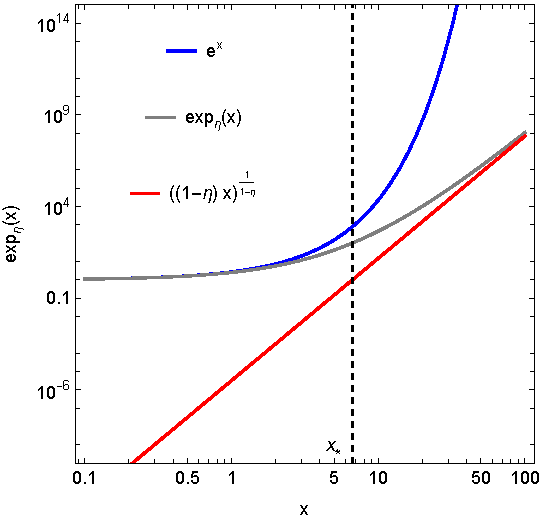
\includegraphics[width=0.9\textwidth]{./crossover.pdf}
\end{center}
\captionof{figure}{\small \helveticanarrow \label{fig-crossover}  Behaviour of $\exp_\eta(x)$ near $\eta=1$.}
\end{Figure}

Adopting the notation in \cite{yamano2002some} to fit the way we usually write the isoelastic utility function, we define the generalised exponential and logarithm as
\begin{align}
\label{eq:exp_eta}
\exp_\eta (x) = & \left\{
\begin{array}{ll} 
\left( 1 + (1-\eta)\,x\right)^\frac{1}{1-\eta} & \text{$0 \leq \eta < 1$}\\
\exp(x) & \text{$\eta=1$}
\end{array}
\right. \\
\label{eq:log_eta}
\log_\eta (x) = & \left\{
\begin{array}{ll} 
\frac{1}{1-\eta}\left( x^{1-\eta} -1 \right) &  \text{$0 \leq \eta < 1$}\\
\log(x) & \text{$\eta=1$}
\end{array}
\right. .
\end{align}
Both $\exp_\eta(x)$ and $\log_\eta(x)$ smoothly converge to the usual exponential and logarithm as $\eta \to 1$. In what follows it will be useful to characterise the behaviour near $\eta=1$ in a bit more detail. It is clear that for fixed $\eta<1$, the leading asymptotic behaviour of $\exp_\eta(x)$ for large $x$ is given by
\begin{align*}
\exp_\eta(x) &\sim (1 - \eta)^\frac{1}{1-\eta}\,x^\frac{1}{1-\eta}.
\end{align*}
When $\eta \to 1$, this expression goes to zero for any fixed $x$. It clearly does not reproduce the exponential asymptotic which we know is the correct large $x$ behaviour for $\eta = 1$. The order of limits matters: to get the correct large $x$ behaviour we must take the limit $\eta \to 1$ {\em before} the limit $x \to \infty$. This behaviour is illustrated in Figure \ref{fig-crossover}: as $\eta \to 1$, $\exp_\eta(x)$ becomes close to $\exp(x)$ for smaller values of $x$ but diverges as $x$ grows. There is no true crossover but we can estimate a characteristic scale as the minimum value of the ratio of terms
\begin{align*}
x_* = \argmin_{x} \frac{\mathrm{e}^x}{ (1 - \eta)^\frac{1}{1-\eta}\,x^\frac{1}{1-\eta}  },
\end{align*}
for which some calculations give
\begin{align}
\label{eq-crossover}
x_* = \frac{1}{1-\eta},
\end{align}
Thus as $\eta \to 1$, the characteristic scale $x_*$  goes to $\infty$ and $\exp_\eta(x)$ converges to $\exp(x)$ from below and from left to right. 

Following \cite{carr2022generalized} we define the generalised compounding operator, $\otimes$, as
\begin{align}
x \otimes y = & \exp_\eta\left[ \log_\eta(x )+ \log_\eta(y)\right].
\end{align}
An $\eta$-compounding process with growth factor, $g$, is one where the initial value is $\eta$-compounded by $g$ at each step:
\begin{align}
x_{t+1} =& x_t \otimes g,
\end{align}
with $x_0 = X_0$. For $T\geq 1$, we have
\begin{align}
\nonumber x_T = & X_0 \otimes  \underbrace{  g\otimes \ldots \otimes g}_{T\text{-times}}\\
\nonumber =&  X_0 \otimes \exp_\eta \left[  \underbrace{  \log_\eta(g)+ \ldots + \log_\eta(g)}_{T\text{-times}}\right]\\
\label{eq:deterministic}=& X_0 \otimes \exp_\eta\left[\log_\eta(g)\,T \right].
\end{align}
From this we see that the growth rate (the quantity with a dimension of $\text{time}^{-1}$) is $\log_\eta(g)$. From Eq.~(\ref{eq:exp_eta}), we see that $\exp_\eta(x)$ is only well defined for
\begin{align*}
x \geq & -\frac{1}{1-\eta} &  \text{$0 \leq \eta < 1$}\\
x >  & -\infty & \text{$\eta=1$}.
\end{align*}
Hence, for general values of $\eta \neq 1$, Eq.~(\ref{eq:deterministic}) is only well-defined for all $T \geq 1$ if $\log_\eta(g) >0$. This implies that $g\geq 1$. 
Some confusion can arise for some rational values of $\eta$ for which the branch point of Eq.~(\ref{eq:exp_eta}) at $x = -\frac{1}{1-\eta}$ disappears. 
For example, if $\eta=\frac{1}{2}$, we have
\begin{align*}
x_T =& \exp_\frac{1}{2}\left[\log_\frac{1}{2}(X_0) + T \log_\frac{1}{2} (g)\right]\\
=& \left[ \sqrt{X_0} + \frac{T}{2}\,\log_\frac{1}{2} (g) \right]^2.
\end{align*}
Although this is well defined for all $T$ even when $\log_\frac{1}{2} (g) <0$, it is not continuously reachable from $\eta = \frac{1}{2} \pm \epsilon$.
Furthermore, this results in an unnatural model where a negative growth rate corresponds to increasing $x_T$. 
In what follows we will respect the constraint $g \geq 1$ in order to avoid such pathologies.


\section{The $\eta$-compounding random walk}
We are interested in studying the $\eta$-compounding random walk in discrete time. At each step, there are now two possible growth factors, $g+r$ and $g-r$, which  we assume occur with equal probability: 
\begin{align}
\label{eq-etaRandomWalk}
x_{t+1} = \left\{ 
\begin{array}{ll}
x_t \otimes \left(g +r \right) & \text{with probability $\frac{1}{2}$}\\
x_t \otimes \left(g - r \right)  & \text{with probability $\frac{1}{2}$}.
\end{array}
\right.
\end{align}
with $x_0 = X_0$.
In order to keep everything well-defined we need $g-r > 1$, assuming that $g>0$ and $r>0$.

We can generalise some of the calculations for the multiplicative random walk in \cite{redner1990random} to the $\eta$-compounding random walk.  
If, after playing $T$ rounds of the game, we experience $n$ ``wins" (and $T-n$ "losses"), then $x_T$ will take the value
\begin{align*}
x_T =  &X_0\otimes \underbrace{g_1\otimes \ldots \otimes g_1}_{n\text{-times}} \otimes \underbrace{g_2\otimes \ldots \otimes g_2}_{T-n\text{-times}} \\
=& X_0\otimes\exp_\eta\left[n\,\log_\eta(g_1)\right]\! \otimes \!\exp_\eta\left[(T\!-\!n) \log_\eta(g_2) \right]\\
=& X_0\otimes \exp_\eta\left[ n\,\log_\eta(g_1) + (T\!-\!n)\log_\eta(g_2) \right],
\end{align*}
where for brevity we write $g_1 = g+r$ and $g_2 = g-r$.
The probability of this value is
\begin{align}
\label{eq:binomialDistr}
p(n) = {T \choose n} \left(\frac{1}{2}\right)^T,
\end{align}
where ${T \choose n}$ is the binomial coefficient -  the number of ways in which $n$ wins can occur in a sequence of $T$ rounds of the game.
The expectation value of $x_T$ is therefore
\begin{align}
\nonumber \mathbb{E}\left[x_T \right] =& \sum_{n=0}^T  {T \choose n} \left(\frac{1}{2}\right)^T  X_0\otimes\exp_\eta\left[ n\,\log_\eta(g_1) \right.\\
\nonumber & \left. + (T-n)\log_\eta(g_2) \right]\\
\nonumber =&   \frac{1}{2^T} \sum_{n=0}^T  {T \choose n} \left[X_0^{1-\eta } -T + n g_1^{1-\eta }\right.\\
\nonumber &\left. + (T-n) g_2^{1-\eta }\right]^{\frac{1}{1-\eta }}\\
\label{eq-expectationxT} =&  \frac{1}{2^T} \sum_{n=0}^T  {T \choose n} \left[X_0^{1-\eta }  +G_2 T + (G_1-G_2) n \right]^{\frac{1}{1-\eta }},
\end{align}
where we write $G_{1,2} = g_{1,2}^{1-\eta}-1$  to keep the notation compact.

\section{Exact expectation value for $\eta=\frac{1}{2}$}

This sum in Eq.~(\ref{eq-expectationxT}) can be done exactly at least for the case $\eta = \frac{1}{2}$ where we have
\begin{align*}
 \mathbb{E}\left[x_T \right] =& \frac{1}{2^T} \sum_{n=0}^T  {T \choose n} \left[\sqrt{X_0}  +G_2 T + (G_1-G_2) n \right]^2.
\end{align*}
After expanding the square in the summand and using Eqs.~(\ref{eq:binomialSum0})-(\ref{eq:binomialSum2}) some algebra leads to
\begin{align*}
 \mathbb{E}\left[x_T \right] =& \frac{1}{4} (G_1+G_2)^2\, T^2 \\
 & + \left[\frac{1}{4}(G_1-G_2)^2 + \sqrt{X_0} (G_1+G_2)\right]\,T\\
 & +X_0.
\end{align*}
In the original notation this is:
\begin{align}
\label{eq:expectationExact} \mathbb{E}\left[x_T\right] =& \frac{1}{4}\left(\sqrt{g+r}+\sqrt{g-r}-2\right)^2\,T^2 \\
\nonumber &+ \left[ (\sqrt{g+r}+\sqrt{g-r}-2) \sqrt{X_0} \right.\\
\nonumber & \left.+ \frac{1}{4}(\sqrt{g+r}-\sqrt{g-r})^2\right]\,T\\
\nonumber &+ X_0.
\end{align}
For large  $T$ we find
\begin{align}
\label{eq:ExLargeT}
\mathbb{E}\left[x_T \right]  \sim & \frac{1}{4} \left( \sqrt{g+r} + \sqrt{g-r} -2\right)^2\, T^2.
\end{align}


\section{Most likely value for the $\eta$-compounding random walk}
The {\em most likely} value of $x_T$ can be found by finding $n^*$,  the value of $n$ that maximises the probability, Eq.~(\ref{eq:binomialDistr}). This is
\begin{align*}
n^* =& \argmax_{n} {T \choose n}\\
=& \frac{T}{2}.
\end{align*}
Thus the most likely value of $x_T$ is
\begin{align}
\nonumber \widetilde{x}_T =& X_0\otimes\exp_\eta\left[ \frac{T}{2}\,\left(\log_\eta(g+r) +\log_\eta(g-r)\right)\right]\\
\label{eq:typicalxT} =&\left(\text{X}_0^{1-\eta} + \left((g+r)^{1-\eta }+(g-r)^{1-\eta }-2\right)\, \frac{T}{2} \right)^\frac{1}{1-\eta}.
\end{align}
For large $T$, we find
\begin{align}
\widetilde{x}_T \sim & \left(\frac{1}{2}  \left((g+r)^{1-\eta }+(g-r)^{1-\eta }-2\right)\right)^\frac{1}{1-\eta} \, T^\frac{1}{1-\eta}.
\end{align}
Note that for $\gamma=\frac{1}{2}$, this agrees with Eq.~(\ref{eq:ExLargeT}) which suggests that for the $\frac{1}{2}$-compounding random walk, the expected value is representative. For $\eta=\frac{1}{2}$, it turns out that the difference between the expected value and the most likely value is sub-leading in $T$:
\begin{align}
\label{eq:difference}\mathbb{E}\left[x_T \right] -  \widetilde{x}_T = \frac{1}{2} T \left(g-\sqrt{g-r} \sqrt{g+r}\right)
\end{align}

\section{Time-averaged growth rate}
From Eq.~(\ref{eq-etaRandomWalk}), the quantity $y_t = \log_\eta x_t$ follows a simple additive random walk:
\begin{align}
\label{eq-addRandomWalk}
y_{t+1} = \left\{ 
\begin{array}{ll}
y_t + a& \text{with probability $\frac{1}{2}$}\\
y_t + b  & \text{with probability $\frac{1}{2}$},
\end{array}
\right.
\end{align}
where 
\begin{align*}
a =& \log_\eta (g+r)\\
b = & \log_\eta (g-r). 
\end{align*}
If, after playing $T$ rounds of the game, we experience $n$ ``wins" (and $T-n$ "losses"), then $y_T$ will take the value
\begin{align*}
y_T =  n\, a + (T-n)\,b.
\end{align*}
The corresponding probability is again given by Eq.~(\ref{eq:binomialDistr}). 
The expectation value of $y_T$ is 
\begin{align}
\nonumber \mathbb{E}\left[y_T \right] =& \sum_{n=0}^T  {T \choose n} \left(\frac{1}{2}\right)^T  \left[ n\, a + (T-n)\,b \right] \\
\nonumber  = & \frac{T}{2} \left( a \sum_{n=0}^T {T \choose n} \,n + b \sum_{n=0}^T {T \choose n} \,(T-n)\right)\\
\nonumber =&  \frac{T}{2} \left(a  + b \right)\\
\label{eq-expectationyT} =&   \frac{T}{2} \left(\log_\eta(g+r)  + \log_\eta(g-r) \right).
\end{align}
where the second-but-last line follows from the identity Eq.~(\ref{eq:binomialSum1}).
Thus the time averaged growth rate corresponds to the growth rate of the most likely trajectory.
We then find that
\begin{align}
\nonumber \exp_\eta \left( \mathbb{E}\left[\log_\eta(x_T) \right]\right) = & \exp_\eta \left[  \frac{T}{2} \left(\log_\eta(g+r)  + \log_\eta(g-r) \right).\right]\\
= & \left(\frac{1}{2}  \left((g-r)^{1-\eta }+(g+r)^{1-\eta }-2\right)\right)^\frac{1}{1-\eta} \, T^\frac{1}{1-\eta}.
\end{align}

\begin{Figure}
\begin{center}
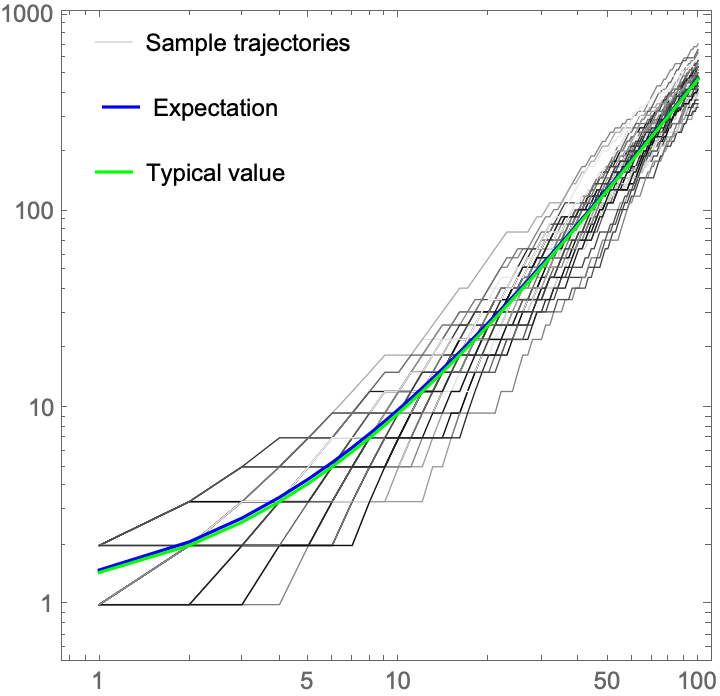
\includegraphics[width=0.9\textwidth]{./sample-trajectories.png}
\end{center}
\captionof{figure}{\small \helveticanarrow \label{fig-trajectories}  Some sample trajectories for $\eta=\frac{1}{2}$ with $g=\frac{3}{2}$ and $r=\frac{1}{2}$.}
\end{Figure}

\section{Exact results for $\eta=\frac{2}{3}$}

Similar calculations to $\eta=\frac{1}{2}$ with a lot more algebra were done by H. Reynolds for $\eta = \frac{2}{3}$. 
The expectation value is
\begin{align}
\label{eq:expectationExact2} \mathbb{E}\left[x_T\right] =& \frac{1}{8}\left( G_1+G_2\right)^3\,T^3 \\
\nonumber &+ \frac{3}{8} \left(G_1+G_2\right) \left[(G_1-G_2)^2 \vphantom{X_0^\frac{1}{3} }  \right.\\
\nonumber & \left.+ 2 X_0^\frac{1}{3} (G_1+G_2)\right]\,T^2\\
\nonumber & + \frac{3}{4} X_0^\frac{1}{3} \left[2 X_0^\frac{1}{3} (G_1+G2) \right.\\
\nonumber & + \left.(G_1-G_2)^2  \vphantom{X_0^\frac{1}{3} } \right]\,T\\
\nonumber &+ X_0.
\end{align}
The most likely value is
\begin{align}
\label{eq:mostLikely2} \widetilde{x}_T =& \frac{1}{8}\left( G_1+G_2\right)^3\,T^3 \\
\nonumber &+ \frac{3}{4} X_0^\frac{1}{3} (G_1+G_2)^2\,T^2\\
\nonumber & + \frac{3}{2} X_0^\frac{2}{3}  (G_1+G2) T\\
\nonumber &+ X_0.
\end{align}
The difference between the two now grows quadratically in time:
\begin{align}
\label{eq:difference2}\mathbb{E}\left[x_T \right] -  \widetilde{x}_T &= \frac{3}{8} (G_1+G_2)(G_1-G_2)^2\, T^2\\
\nonumber&+ \frac{3}{4} X_0^\frac{1}{3} (G_1-G_2)^2\,T.
\end{align}
\end{multicols}

\section{Review of results for multiplicative case, $\eta = 1$}
In this section, I summarise the results of Redner \cite{redner1990random}  for the general multiplicative random walk 
\begin{align}
\label{eq-multiplicativeRandomWalk}
x_{t+1} = \left\{ 
\begin{array}{ll}
x_t \, z_1 & \text{with probability $p$}\\
x_t \, z_2  & \text{with probability $q=1-p$}.
\end{array}
\right.
\end{align}
with $x_0 = 1$.
The expected value after $T$ steps is
\begin{align}
 \mathbb{E}\left[x_T \right] =& X_0 \sum_{n=0}^T  P(n,T) \, z_1^n z_2^{T-n},
\end{align}
where $P(n,T)$ is the binomial distribution,
\begin{align}
P(n, T) = {T \choose n}\, p^n q^{T-n} =  \frac{T!}{(T-n)!\,n!}\, p^n q^{T-n}.
\end{align}
The expected value can be calculated directly as
\begin{align}
\nonumber  \mathbb{E}\left[x_T \right] =&X_0 \sum_{n=0}^T  {T \choose n} \, (p\,z_1)^n (q z_2)^{T-n}\\
\label{eq-Ex-mult-exact}& = X_0 \left(p z_1 + q z_2 \right)^T,
\end{align}
which follows from the binomial theorem. The growth factor for the expected value is the
arithmetic mean of $z_1$ and $z_2$.

Note that the typical value of $x_T$ occurs for $n = p\,T$ and is given by
\begin{align}
\label{eq-typical-value-mult}
\widetilde{x}_T = X_0\,z_1^{p\,T}\,z_2^{(1-p)\,T} = X_0\,\left(z_1^p\,z_2^q \right)^T.
\end{align}
The growth factor for the typical value is the geometric mean of $z_1$ and $z_2$.

For what follows, it is instructive to learn how to recover the large $T$ behaviour of $\mathbb{E}\left[x_T \right]$ without directly evaluating the sum.
The idea is to take a continuum limit in which the sum can be written as an integral which can then be approximated using methods of asymptotic analysis.
Starting with the binomial distribution, we use Stirling's approximation,
\begin{align}
n! = \sqrt{2 \pi n} \left( \frac{n}{\mathrm{e}}\right)^n\left(1 + \frac{1}{12\,n} + \mathcal{O}\left(\frac{1}{n^2}\right)\right),
\end{align}
to approximate the factorials. We then take the continuum limit, $T\to \infty$ with $x=\frac{n}{T}$ fixed,
 to obtain 
\begin{align}
\label{eq-binomial-distribution-cts-limit}
P_\text{cont}(x, T) = \left\{
\begin{array}{ll}
\frac{1}{\sqrt{2 \pi T \,x\,(1-x)}}\,\mathrm{e}^{T\,\phi(x)}\left(1 + \frac{1}{12}\left( 1-\frac{1}{x} - \frac{1}{1-x}\right) \frac{1}{T}   + \mathcal{O}\left(\frac{1}{T^2}\right)\right) & 0 < x< 1\\
0 & \text{otherwise}
\end{array}
\right.
\end{align}
where
\begin{align}
\label{eq-phi}
\phi(x) =    x \log(p) +  (1 - x) \log (q)  - x \log(x) -  (1 - x) \log(1 - x).
\end{align}
Writing $\mathbb{E}\left[x_T \right]$ in the form
\begin{align*}
\mathbb{E}\left[x_T \right] &=   X_0 \sum_{n=0}^T  P(n,T) \, \left(z_1^\frac{n}{T} z_2^{1-\frac{n}{T}}\right)^T,
\end{align*}
we can replace the sum by an integral in the continuum limit to obtain
\begin{align}
\nonumber \mathbb{E}\left[x_T \right] &=   T\,X_0\, \int_{-\infty}^\infty P_\text{cont}(x, T)\,\left( z_1^x\,z_2^{1-x}\right)^T\\ 
\nonumber & = T\,X_0\, \int_{-\infty}^\infty P_\text{cont}(x, T)\,\mathrm{e}^{T\left(x\log z_1 + (1-x)\log z_2 \right)}\\
\label{eq-Ex-mult1} & = T^\frac{1}{2} X_0  \int_{-\infty}^\infty  \frac{d x}{\sqrt{2 \pi \,x\,(1-x)}}\,\mathrm{e}^{T\,\widetilde{\phi}(x)}\left(1 + \frac{1}{12}\left( 1-\frac{1}{x} - \frac{1}{1-x}\right) \frac{1}{T}   + \mathcal{O}\left(\frac{1}{T^2}\right)\right) \, \chi_{\left[0, 1\right]}(x),
\end{align}
where 
\begin{align}
\widetilde{\phi}(x) =  x \log(p) +  (1 - x) \log (q)  - x \log(x)  (1 - x) \log(1 - x) + x \log z_1 +  (1-x)\log z_2.
\end{align}
$\mathbb{E}\left[x_T \right] $ can therefore be broken up into a series of integrals,
\begin{align}
\label{eq-Ex-mult2}
\mathbb{E}\left[x_T \right] &= T^\frac{1}{2}\, \mathcal{I}_1(T) + T^{-\frac{1}{2}} \mathcal{I}_2(T) +\ldots 
\end{align}
each of which is of the form
\begin{align}
\label{eq-Fk-mult}
 \mathcal{I}_k(T) & =  X_0\, \int_{-\infty}^\infty\, F_k(x) \,\mathrm{e}^{T\,\widetilde{\phi}(x)}\, d x,
\end{align}
with
\begin{align}
\label{eq-ampl0} F_0(x) &=  \frac{1}{\sqrt{2 \pi \,x\,(1-x)}} \, \chi_{\left[0, 1\right]}(x)\\
\label{eq-ampl1} F_1(x) &=  \frac{1}{12}\, \frac{1}{\sqrt{2 \pi \,x\,(1-x)}} \, \left( 1-\frac{1}{x} - \frac{1}{1-x}\right)\,\chi_{\left[0, 1\right]}(x).
\end{align}
Integrals of the form
\begin{align}
\label{eq-LaplaceIntegral0}
I(T) = \int_{-\infty}^{\infty} F(x)\,\mathrm{e}^{T\,\phi(x)}\, dx,
\end{align}
are standard Laplace integrals. Such integrals have the following asymptotic behaviour as $T \to \infty$ \cite{bender2013advanced}:
\begin{align}
\label{eq-LaplaceAsymptoticFormula}
I(T) \sim \sqrt{\frac{2\pi }{-T\,\phi^{\prime\prime}(x^*)}}\,\mathrm{e}^{T \,\phi(x^*)}\left(F(x^*)+B(x^*) T^{-1}+\mathcal{O}\left(T^{-2}\right)\right),
\end{align}
where $x^*$ is the maximum of $\phi(x)$ and
\begin{align}
\label{eq-LaplaceAsymptoticFormulaLeadingCorrection}
B(x^*) &=  - \frac{F^{\prime\prime}(x^*)}{2\, \phi^{\prime\prime}(x^*)} 
                 + \frac{F(x^*) \phi^{\prime\prime\prime\prime}(x^*)}{8\,\phi^{\prime\prime}(x^*)^2}
                 + \frac{F^\prime(x^*) \phi^{\prime\prime\prime}(x^*)}{2\,\phi^{\prime\prime}(x^*)^2}
                 - \frac{5\,F(x^*) \phi^{\prime\prime\prime}(x^*)^2}{24\,\phi^{\prime\prime}(x^*)^3}
\end{align}
To find the maximum of $\widetilde{\phi}$ we solve
\begin{align*}
\widetilde{\phi}^\prime (x^*) &= 0\\
 \log p z_1 - \log q z_2 - \log x^* + \log (1-x^*) &= 0\\
 \log \left( \frac{p z_1}{q z_2} \frac{1-x^*}{x^*}\right) = 0
\end{align*}
which gives
\begin{align}
\label{eq-xStar-mult}
x^* = \frac{\xi}{1+\xi} \hspace{1.0cm}\text{with }\xi = \frac{p z_1}{q z_2}.
\end{align}
The second derivative is
\begin{align*}
\widetilde{\phi}^{\prime\prime} (x) &= -\frac{1}{x} - \frac{1}{1-x}.
\end{align*}
We can now use Eq.~(\ref{eq-LaplaceAsymptoticFormula}) to extract the leading order behaviour
of  $\mathbb{E}\left[x_T \right]$ in Eq.~(\ref{eq-Ex-mult2}) from the leading order behaviour of $\mathcal{I}_0(T)$. The quantities required are:
\begin{align}
\widetilde{\phi} (x^*) & = \log\left( p z_1 + q z_2 \right)\\ 
\widetilde{\phi}^{\prime\prime} (x^*) &= - \frac{(p z_1 + q z_2)^2}{ p q z_1 z_2}\\
F_0(x^*) & = \frac{p z_1 + q z_2}{\sqrt{2 \pi p q z_1 z_2 }}
\end{align}
Putting all the bits together in  Eq.~(\ref{eq-LaplaceAsymptoticFormula}) we get the leading order asymptotic behaviour
\begin{align}
\nonumber \mathbb{E}\left[x_T \right] &\sim T^\frac{1}{2} \, X_0 \sqrt{\frac{2 \pi p q z_1 z_2}{T (p z_1 + q z_2)^2}} \,\mathrm{e}^{T\, \log\left( p z_1 + q z_2 \right)}\,  \frac{p z_1 + q z_2}{\sqrt{2 \pi p q z_1 z_2 }}\\
&= X_0\,  (p z_1 + q z_2)^T.
\end{align}
We recover the exact result, Eq.~(\ref{eq-Ex-mult-exact}). This tells us that the sub-leading terms in the expansion (\ref{eq-Ex-mult2}) must vanish.
This can either be because they are all zero for some reason or because the corrections coming from using Stirlings formula to approximate the binomial distribution by its continuum limit in Eq.~(\ref{eq-binomial-distribution-cts-limit}) cancel the higher order terms in the Laplace integral in Eq.~(\ref{eq-LaplaceAsymptoticFormula}).
With some help from Mathematica we can evaluate these terms to show that it is the latter.
The sub-leading  $\mathcal{O}(T^{-1})$ contribution in Eq.~(\ref{eq-LaplaceAsymptoticFormula}) to $\mathcal{I}_0(T)$ is
\begin{align*}
\frac{ (p z_1 + q z_2)\left(p^2 z_1^2 + p q z_1 z_2 + q^2 z_2^2 \right)}{12 \sqrt{2 \pi  (p q z_1 z_2)^3}}
\end{align*}
The  leading  $\mathcal{O}(T^{-1})$ contribution to $\mathcal{I}_1(T)$ in Eq.~(\ref{eq-Ex-mult2}) is
\begin{align*}
- \frac{ (p z_1 + q z_2)\left(p^2 z_1^2 + p q z_1 z_2 + q^2 z_2^2 \right)}{12 \sqrt{2 \pi  (p q z_1 z_2)^3}}.
\end{align*}
Thus we learn that to correctly calculate the sub-leading behaviour, we need to account for cancellations between the corrections to the continuum limit of the binomial distribution and the corrections to the Laplace formula.

\section{Asymptotic analysis for $ 0 < \eta < 1$}

We can adapt the analysis above to calculate the asymptotic behaviour for $0 \leq \eta \leq 1$. Write the random $\eta$-compounding random walk in its more general form as
\begin{align}
\label{eq-etaRandomWalk2}
x_{t+1} = \left\{ 
\begin{array}{ll}
x_t \otimes z_1 & \text{with probability $p$}\\
x_t \otimes z_2  & \text{with probability $q=1-p$}.
\end{array}
\right.
\end{align}
with $x_0 = 1$.
Working through the definition of $\eta$-compounding we can write the expected value after $T$ steps as
\begin{align}
\label{eq-expected-value-eta}
 \mathbb{E}\left[x_T \right]  =  \sum_{n=0}^T  P(n,T) \,G(n, T, \eta)
\end{align}
where
\begin{align}
G(n, T, \eta) &= \left[ n z_1^{1-\eta} + (T-n) z_2^{1-\eta} -T + X_0^{1-\eta}\right]^\frac{1}{1-\eta}
\end{align}
The typical value is
\begin{align}
\nonumber \widetilde{x}_T &= \left( p T z_1^{1-\eta} + (1-p) T z_2^{1-\eta} - T+X_0^{1-\eta} \right)^\frac{1}{1-\eta}\\
\label{eq-typical-value-eta}&=  \left( p T z_1^{1-\eta} +  q T z_2^{1-\eta} - T+X_0^{1-\eta} \right)^\frac{1}{1-\eta}\\
\nonumber &= \exp_\eta\left[\log_\eta(X_0) + T \left(p \log_\eta(z_1) + q \log_\eta(z_2)\right)\right].
\end{align}
Note that this expression has a regular limit as $\eta \to 1$:
\begin{align}
\label{eq-typical-value-mult}
\lim_{\eta \to 1}  \left( p T z_1^{1-\eta} +  q T z_2^{1-\eta} - T+X_0^{1-\eta} \right)^\frac{1}{1-\eta} &= X_0\,\left( z_1^p z_2^q \right)^T,
\end{align}
which agrees with Eq.(\ref{eq-typical-value-mult}). However, we notice that in order to reach this limit,
we must include the $X_0$ term which is sub-leading with respect to $T$. In order to recover the large time behaviour as $\eta$ approaches the multiplicative case, the order of limits matters: we must take $\eta \to 1$ {\em before} taking $T \to \infty$. If we take $X_0=1$ so that $\log_\eta(X_0)=0$  and refer back to Eq.~(\ref{eq-crossover}), we find that as $\eta \to 1$ the typical value tracks close to the multiplicative result, Eq.~(\ref{eq-typical-value-mult}), for 
\begin{align}
T &< \frac{1}{(1-\eta)\left(p \log(z_1) + q \log(z_2) \right)},
\end{align}
before crossing over to the $T^\frac{1}{1-\eta}$ power law behaviour.  Here we have neglected higher order correction terms in $1-\eta$.

To obtain the large $T$ behaviour of the expected value, $\mathbb{E}\left[x_T \right] $,  start by writing
Eq.~(\ref{eq-expected-value-eta}) in the form
\begin{align*}
 \mathbb{E}\left[x_T \right]  =  \sum_{n=0}^T  P(n,T) \,T^\frac{1}{1-\eta}\, \left[ \left(\frac{n}{T}\right) z_1^{1-\eta} + \left(1-\frac{n}{T}\right) z_2^{1-\eta} -1 + \frac{X_0^{1-\eta}}{T}\right]^\frac{1}{1-\eta}.
\end{align*}
We again take the continuum limit, $T\to \infty$ with $x=\frac{n}{T}$ fixed, and replace the sum with an integral in Eq.~(\ref{eq-expected-value-eta}) to obtain
\begin{align}
\nonumber \mathbb{E}\left[x_T \right] & =  T^{1+\frac{1}{1-\eta}}\, \int_{-\infty}^\infty P_\text{cont}(x, T)\,  \left[ x z_1^{1-\eta} + \left(1-x\right) z_2^{1-\eta} -1 + \frac{X_0^{1-\eta}}{T}\right]^\frac{1}{1-\eta}\,d x\\
  \label{eq-EV-eta}&= T^{\frac{1}{1-\eta}+\frac{1}{2}}  \int_{-\infty}^\infty F(x,T) \,\mathrm{e}^{T\,\phi(x)}\left(1 + \frac{1}{12}\left( 1-\frac{1}{x} - \frac{1}{1-x}\right) \frac{1}{T}   + \mathcal{O}\left(\frac{1}{T^2}\right)\right) \, \chi_{\left[0, 1\right]}(x) \, dx,
\end{align} 
where
\begin{align*}
F(x,T) = \frac{1}{\sqrt{2 \pi \,x\,(1-x)}} \,  \left[ x z_1^{1-\eta} + \left(1-x\right) z_2^{1-\eta} -1 + \frac{X_0^{1-\eta}}{T}\right]^\frac{1}{1-\eta}
\end{align*}
and $\phi(x)$ is given by Eq.~(\ref{eq-phi}). Now expand $F(x,T)$ in powers of $\frac{1}{T}$:
\begin{align*}
F(x,T) =  \frac{1}{\sqrt{2 \pi \,x\,(1-x)}} \,   \sum_{k=0}^\infty {\frac{1}{1-\eta} \choose k} \left(x z_1^{1-\eta} + \left(1-x\right) z_2^{1-\eta} -1 \right)^{\frac{1}{1-\eta}-k}\,X_0^{(1-\eta)\,k}\frac{1}{T^k}
\end{align*}
If we keep only the leading term in Eq.~(\ref{eq-EV-eta}), and exchange the order of integration and summation we get
\begin{align}
\label{eq-EV-eta-2}
\mathbb{E}\left[x_T \right] & =  T^{\frac{1}{1-\eta}+\frac{1}{2}}   \sum_{k=0}^\infty {\frac{1}{1-\eta} \choose k}  \mathcal{F}_k(T) \left(\frac{X_0^{1-\eta}}{T}\right)^k,
\end{align}
where the $\mathcal{F}_k(T)$ are integrals whose asymptotic behaviour for large $T$ can be obtained directly using the Laplace method:
\begin{align}
\mathcal{F}_k(T) &=   \int_{-\infty}^\infty    \frac{dx}{\sqrt{2 \pi \,x\,(1-x)}}\,\left(x z_1^{1-\eta} + \left(1-x\right) z_2^{1-\eta} -1 \right)^{\frac{1}{1-\eta}-k}\, \mathrm{e}^{T\,\phi(x)} \\
&\sim \frac{1}{\sqrt{T}}\, \left( p z_1^{1-\eta} + q z_2^{1-\eta} -1\right)^{\frac{1}{1-\eta}-k}.
\end{align}
Putting this back into Eq.~(\ref{eq-EV-eta-2}), we get
\begin{align}
\nonumber \mathbb{E}\left[x_T \right] &\sim T^\frac{1}{1-\eta}   \sum_{k=0}^\infty {\frac{1}{1-\eta} \choose k}   \,\left( p z_1^{1-\eta} + q z_2^{1-\eta} -1\right)^{\frac{1}{1-\eta}-k}\,\left(\frac{X_0^{1-\eta}}{T}\right)^k \\
\label{eq-EV-eta-3} &=  T^\frac{1}{1-\eta} \, \left( p z_1^{1-\eta} + q z_2^{1-\eta} -1 + \frac{X_0^{1-\eta}}{T}\right)^\frac{1}{1-\eta} \\
\nonumber &= \widetilde{x}_T.
\end{align}
To leading order, $\mathbb{E}\left[x_T \right] $ coincides with the typical value for large $T$. Note that Eq.~(\ref{eq-EV-eta-3}) behaves exponentially as $\eta \to 1$ as per Eq.~(\ref{eq-typical-value-mult}). However we do not recover the correct growth rate which we know from the exact result Eq.~(\ref{eq-Ex-mult-exact}). Eq.~(\ref{eq-EV-eta-3}) results from adding up an infinite sum of sub-leading contributions but we didn't do this consistently: some sub-leading terms were not included without any justification. To calculate the asymptotic difference between $\mathbb{E}\left[x_T \right] $ and $ \widetilde{x}_T$, we need to consistently account for all the terms of order $\frac{1}{T}$ in Eq.~(\ref{eq-EV-eta}). There are two terms that we neglected: the $\mathcal{O}\left(\frac{1}{T}\right)$ term in Eq.~(\ref{eq-EV-eta}) coming from the correction to Stirling's formula and the $\mathcal{O}\left(\frac{1}{T}\right)$ term that arose when we applied the Laplace method to calculate $\mathcal{F}_0(T)$ (see Eq.~(\ref{eq-LaplaceAsymptoticFormula}) and Eq.~(\ref{eq-LaplaceAsymptoticFormulaLeadingCorrection}) ). As with, the purely multiplicative case, there are cancellations between these two terms at $\mathcal{O}\left(\frac{1}{T}\right)$ so both need to be calculated carefully. If you do this in Mathematica, you end up with the asymptotic formula
\begin{align*}
\mathbb{E}\left[x_T\right] = T^\frac{1}{1-\eta} \left( p Z_1 + q Z_2\right)^\frac{1}{1-\eta} \left[ 1+  
\frac{1}{T}\left( \frac{p q}{2}\frac{\eta}{(1-\eta)^2}\left(\frac{Z_1-Z_2}{pZ_1+q Z_2}\right)^2 + \frac{X_0^{1-\eta}}{1-\eta} \frac{1}{p Z_1+q Z_2}\right)
+ \mathcal{O}\left(\frac{1}{T^2}\right) \right],
\end{align*}
where, to compress the notation, we have defined
\begin{align*}
Z_{1,2} &= z_{1,2}^{1-\eta}-1.
\end{align*}
This formula agrees with the exact results available for $\eta = \frac{1}{2}$ and $\eta=\frac{2}{3}$ for the case $p=\frac{1}{2}$ so we can be fairly confident that we have the correct behaviour.

\section{Uniform asymptotic expansion near $\eta = 1$}

Neglecting the higher order terms in $P_\text{cont}(x,T)$ for now, let us write Eq.~(\ref{eq-EV-eta}) in the form
\begin{align}
\nonumber \mathbb{E}\left[x_T \right] & 
= T^\frac{1}{2}  \int_{-\infty}^\infty \frac{dx}{\sqrt{2 \pi x (1-x)}} \,\mathrm{e}^{T\,\phi(x)+ \frac{1}{\zeta}\log\left[T \left( x (z_1^\zeta - 1) + (1-x) (z_2^\zeta -1) \right) + X_0^{\zeta} \right]}\\
  \label{eq-EV-eta-2}  &= T^\frac{1}{2}  \int_{-\infty}^\infty \frac{dx}{\sqrt{2 \pi x (1-x)}} \,\mathrm{e}^{T\, \left\{\phi(x)+ \frac{1}{\zeta T}\log\left[T \left( x (z_1^\zeta - 1) + (1-x) (z_2^\zeta -1) \right) + X_0^{\zeta} \right]\right\}},
\end{align} 
where we have defined $\zeta = 1 - \eta$ for convenience.
To obtain a uniform asymptotic expansion that (hopefully) remains valid as $\eta \to 1$, we need to introduce the uniformity parameter,
\begin{align}
\label{eq-uniformity-parameter}
\lambda = \zeta \,T,
\end{align}
and then take the limit $T\to\infty$ with $\lambda$ fixed.  This corresponds to a limit where $T$ is large and $\zeta = 1-\eta = \mathcal{O}\left(\frac{1}{T}\right)$. Writing $T=\frac{\lambda}{\zeta}$ inside the $\log$ part of the phase function in Eq.~(\ref{eq-EV-eta-2}) we can write
\begin{align}
  \label{eq-EV-eta-3}  \mathbb{E}\left[x_T \right] & = T^\frac{1}{2}  \int_{-\infty}^\infty \frac{dx}{\sqrt{2 \pi x (1-x)}} \,\mathrm{e}^{T\,\psi_\lambda(x)},
\end{align}
where the new phase function is
\begin{align}
\nonumber \psi_\lambda(x) &=    x \log(p) +  (1 - x) \log (q)  - x \log(x) -  (1 - x) \log(1 - x) \\
\label{eq-psi_lambda} &+  \frac{1}{\lambda}\log\left[\frac{\lambda}{\zeta} \left( x (z_1^\zeta - 1) + (1-x) (z_2^\zeta -1) \right) + X_0^{\zeta} \right].
\end{align}
Eq.~(\ref{eq-EV-eta-3}) is a standard Laplace integral with the phase function parameterised by the (fixed) uniformity parameter, $\lambda$.
The first two derivatives of $\psi_\lambda(x)$ are
\begin{align}
\psi_\lambda^\prime(x) & = 2\, \arctanh(1-2 x) + \log\left(\frac{p}{q}\right) + \frac{z_1^\zeta - z_2^\zeta}{\zeta X_0^\zeta + \lambda\left( x (z_1^\zeta -1) + (1-x)(z_2^\zeta - 1)\right)} \\
\psi_\lambda^{\prime\prime}(x) & = -\frac{1}{x} -\frac{1}{1-x} -  \frac{\lambda(z_1^\zeta - z_2^\zeta)^2}{\left[ \zeta X_0^\zeta + \lambda\left( x (z_1^\zeta -1) + (1-x)(z_2^\zeta - 1)\right)\right]^2}. 
\end{align}
Finding the critical point, $x_\lambda^*$, requires the solution of a transcendental equation which, writing $x = \frac{1}{2}(1- y)$ can be written as
\begin{align}
0=-2 \arctanh(y) + \log\left(\frac{p}{q}\right) + \frac{1}{\frac{\lambda}{2} \left(1 - y \right) + \frac{\zeta X_0^\zeta}{z_1^\zeta - z_2^\zeta}} 
\end{align}
I don''t know how to solve this equation in general but two limiting cases can be considered:

\begin{itemize}
\item{$\mathbf \lambda \to \infty$:\\}
In this case we have
\begin{align*}
0 &= 2 \arctanh(y) + \log\left(\frac{p}{q}\right)\\
\Rightarrow y_\infty^* & = \tanh \left[-\frac{1}{2}\log\left(\frac{p}{q}\right) \right]\\
\Rightarrow x_\infty^* & = \frac{1}{2}\left( 1 -  \tanh \left[-\frac{1}{2}\right]\ \right)\\
&= \frac{\mathrm{e}^{\log\left(\frac{p}{q}\right) }}{1 + \mathrm{e}^{\log\left(\frac{p}{q}\right)} }\\
&= \frac{p}{p+q} = p.
\end{align*}
This is the same critical point we found earlier for the case $\eta <1$.
\item{$\mathbf \lambda \to 0$:\\}
In this case we have:
\begin{align}
\nonumber 0 &= 2 \arctanh(y) + \log\left(\frac{p}{q}\right) + \frac{z_1^\zeta - z_2^\zeta}{\zeta X_0^\zeta}\\
\nonumber \Rightarrow y_\infty^* & = \tanh \left[-\frac{1}{2}\left(\log\left(\frac{p}{q}\right) +  \frac{z_1^\zeta - z_2^\zeta}{\zeta X_0^\zeta}\right) \right]\\
\nonumber \Rightarrow x_\infty^* & = \frac{1}{2}\left( 1 -  \tanh \left[-\frac{1}{2}\left( \log\left(\frac{p}{q}\right) +  \frac{z_1^\zeta - z_2^\zeta}{\zeta X_0^\zeta}\right)\right]\ \right)\\
\Rightarrow x_\infty^* &= \frac{\xi(\zeta)}{1 + \xi(\zeta) }
\end{align}
where
\begin{align}
\label{eq-xi_zeta}
\xi(\zeta) = \frac{p}{q}\,\mathrm{e}^{\frac{z_1^\zeta - z_2^\zeta}{\zeta X_0^\zeta}}.
\end{align}
Note that
\begin{align*}
\lim_{\zeta \to 0} \xi(\zeta) =  \frac{p}{q} \,\mathrm{e}^{\frac{\zeta \left( \log(z_1) - \log(z_2)\right)}{\zeta}} =  \frac{p}{q} \frac{z_1}{z_2},
\end{align*}
so in this limit Eq.~(\ref{eq-xi_zeta}) approaches the critical point Eq.~(\ref{eq-xStar-mult}) which we already found for the case $\eta=1$.
\end{itemize}





\bibliographystyle{plain}
\bibliography{refs}



\end{document}
